\documentclass[aspectratio=1610]{beamer}
\usepackage[utf8]{inputenc}
\usepackage{polski}
\usepackage[T1]{fontenc}
\usepackage{tikz}
\usepackage{tikzducks}
% \usetikzlibrary{decorations.pathmorphing}
\usepackage{multimedia}
\usepackage{graphicx}
\usepackage[
  % justification=centering, 
  font=scriptsize
]{caption}
\captionsetup{singlelinecheck=off}
\captionsetup[figure]{textfont={small}}
\setbeamerfont{caption}{size=\small}
\usepackage{textcomp}
\usepackage{appendixnumberbeamer}
\usepackage{qrcode}
% \usepackage[natbib, language=polish, sorting=none]{biblatex}
% \addbibresource{lio.bib}
\usepackage{hyperref}
%\usepackage[width=\textwidth]{animate}
%\usepackage{chemformula}
\usepackage{sidecap}
\usepackage{multirow}
\usepackage{multicol}
\usepackage{rotating}
\usepackage{anyfontsize} % change font size for semposiwko

% \usepackage{physics}
\usepackage{array}
\usepackage{booktabs}
\usepackage{transparent}
\usepackage{siunitx}
% \usepackage[rightcaption]{sidecap}
\usepackage{eso-pic}

\usepackage{amsmath,amsthm,amssymb}
\DeclareMathOperator{\sgn}{sgn}

\usepackage{listings}
\lstset{
basicstyle=\small\ttfamily,
columns=flexible,
breaklines=true
}

% \usepackage{emoji}
\usepackage{subcaption}
% \usepackage{enumerate}

\usepackage[natbib, sorting=none, style=authoryear]{biblatex}
% \usepackage{bibentry}
\addbibresource{lio.bib}
\renewcommand*{\bibfont}{\scriptsize}

\usefonttheme[onlymath]{serif}

\usetheme{Szeged}
\usecolortheme{whale}
\setbeamercolor{palette primary}{bg=violet!80!black,fg=white}
\setbeamercolor{palette secondary}{bg=violet!60!black,fg=white}
% \definecolor{deepviolet}{RGB}{46,0,79}
% \definecolor{vividpink}{RGB}{255,0,127}
% \setbeamercolor{palette primary}{bg=deepviolet,fg=white}
% \setbeamercolor{palette secondary}{bg=vividpink,fg=white}
\setbeamercolor{palette tertiary}{bg=violet!40!black,fg=white}
\setbeamercolor{palette quaternary}{bg=violet!20!black,fg=white}
\setbeamercolor{structure}{fg=violet!60!black}
% \setbeamertemplate{caption}{\insertcaption}
% \setbeamertemplate{headline}{
%   \begin{beamercolorbox}[wd=.9\paperwidth]{headline}
%     \vspace{1.5ex}
%     \insertsectionnavigationhorizontal
%     \vspace{1.5ex}
%   \end{beamercolorbox}
% }
% \definecolor{violet-dark}{HTML}{4B0082}
% \definecolor{teal}{HTML}{008080}
% \definecolor{amber}{HTML}{FFC107}
% \definecolor{light-grey}{HTML}{F5F5F5}
% \definecolor{charcoal}{HTML}{333333}
% \setbeamercolor{palette primary}{bg=violet-dark, fg=white}
% \setbeamercolor{palette secondary}{bg=teal, fg=white}
% \setbeamercolor{palette tertiary}{bg=amber, fg=charcoal}
% \setbeamercolor{background canvas}{bg=light-grey}
% \setbeamercolor{normal text}{fg=charcoal}
% Główna paleta fioletów
% \definecolor{coolblack}{HTML}{000000}
% \definecolor{coolnavy}{HTML}{14213D}
% \definecolor{coolorange}{HTML}{FCA311}
% \definecolor{coollightgray}{HTML}{E5E5E5}
% \definecolor{coolwhite}{HTML}{FFFFFF}

% % Opcjonalnie: ustawienia kolorów dla Beamera
% \setbeamercolor{normal text}{fg=coolblack,bg=coolwhite}
% \setbeamercolor{structure}{fg=coolorange}
% \setbeamercolor{frametitle}{fg=coolwhite,bg=coolnavy}
% \setbeamercolor{title}{fg=coolwhite,bg=coolnavy}
% \setbeamercolor{item}{fg=coolorange}
% \setbeamercolor{block title}{fg=coolwhite,bg=coolnavy}
% \setbeamercolor{block body}{fg=coolblack,bg=coollightgray}
% \setbeamercolor{palette tertiary}{fg=coolwhite, bg=coolorange}
% \setbeamercolor{palette quaternary}{fg=coolblack, bg=coollightgray}

\linespread{0.8}

\setbeamertemplate{background}%
{%
    \begin{tikzpicture}[remember picture,overlay]{\node[yshift=1.5cm,xshift=-2cm,opacity=0.1] at (current page.south east)
      {
      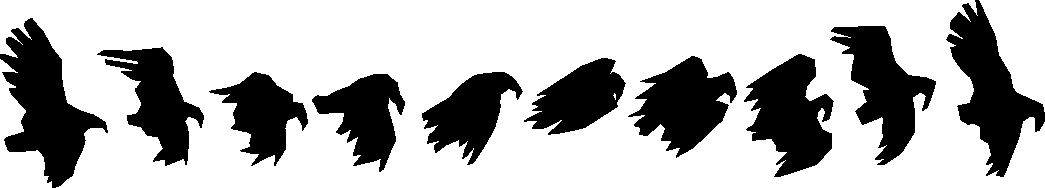
\includegraphics[scale=0.4, angle=25]{ptaki.pdf}
      }
      ;
    \node[yshift=-2cm,xshift=-2cm,opacity=0.1] at (current page.north east)
      {
      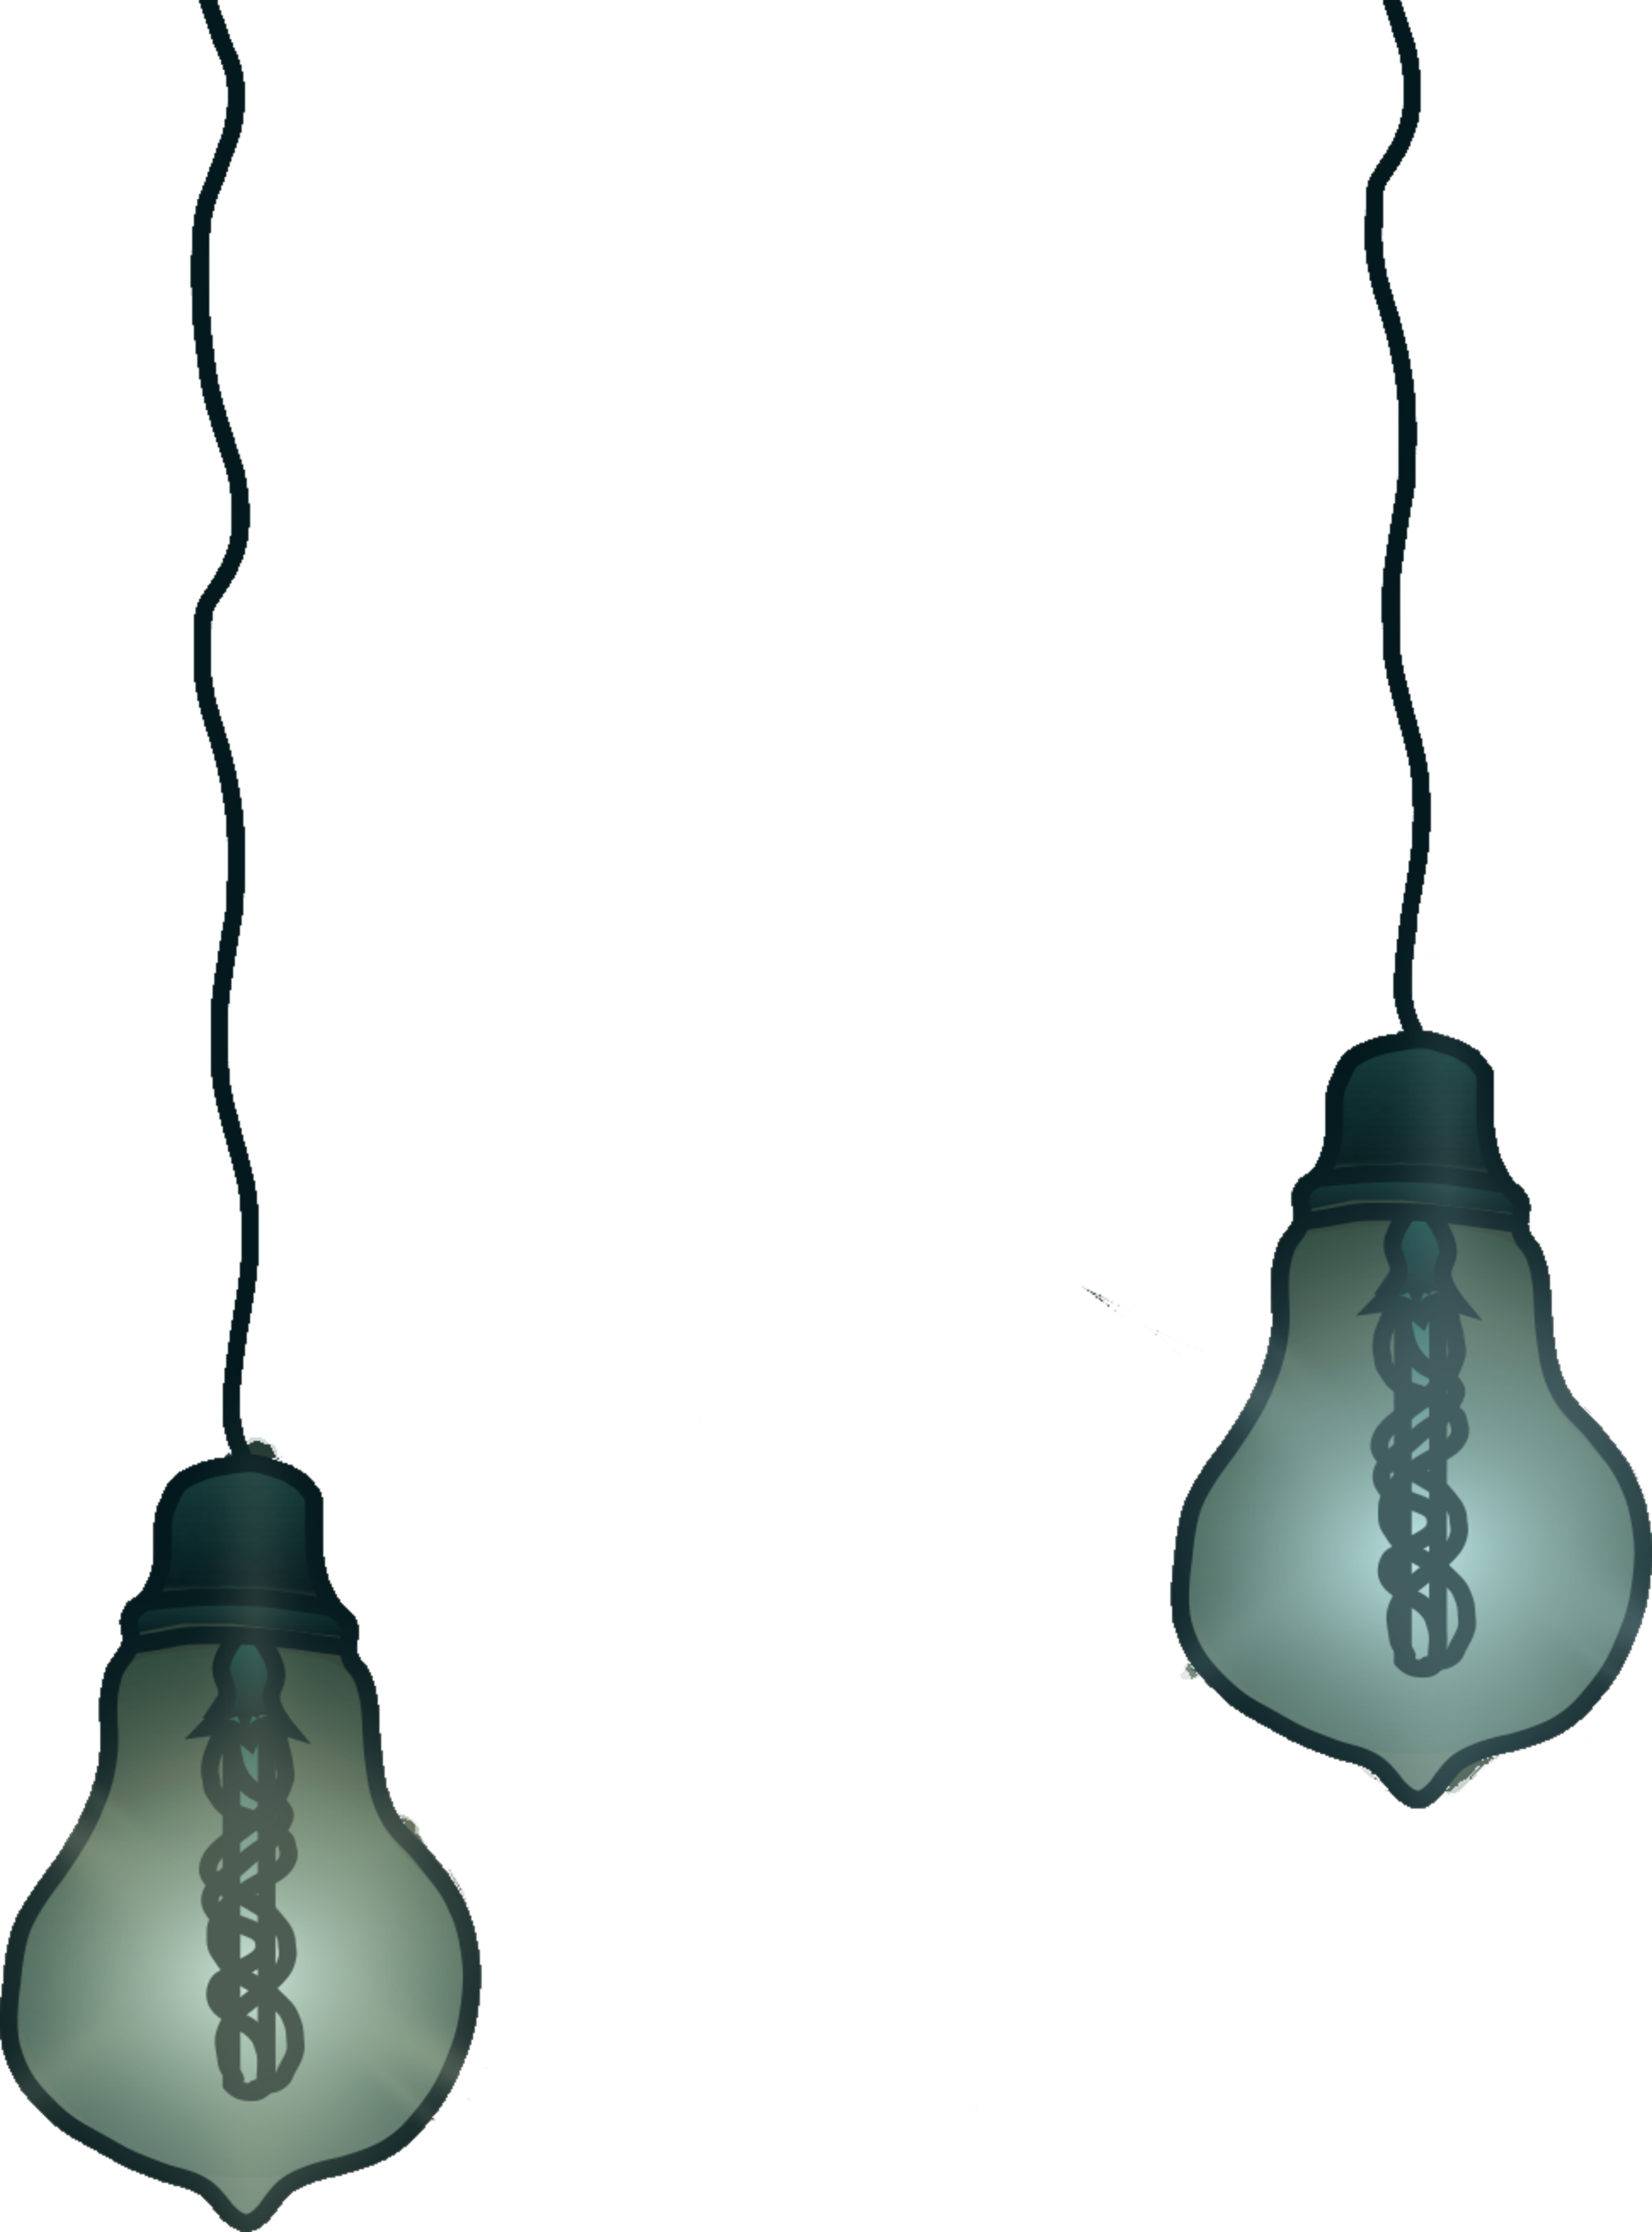
\includegraphics[scale=0.1, angle=0]{zarowki.pdf}
      }
      ;
    \node[yshift=1.0cm,xshift=0.6cm] (logopos) at (current page.south west) {{\begin{tikzpicture}\shuffleducks\duck[signpost=\insertframenumber, \randomhead,scale=.4]\end{tikzpicture}}};
    \pgfmathsetmacro{\progress}{360*(\insertframenumber)/(\inserttotalframenumber)};
    \draw[line width=0.2*3pt] ([xshift=0.55cm] logopos)  arc[radius=0.55cm, start angle=0, end angle=\progress];
    \fill ([shift={(\progress:0.55cm)}] logopos) circle(1pt);

    }
        \end{tikzpicture}
    
}

\newcommand{\SeMPowisko}{%
\large S\normalsize%
\kern-.3em \lower.2ex\hbox{e}%
\lower.2ex\hbox{\large M\normalsize}%
\kern-.1em \raise.1ex\hbox{\large P\normalsize}%
\kern-.3em \lower.2ex\hbox{o}%
\kern-.2em \raise.2ex\hbox{w}%
\lower.2ex\hbox{i}%
s%
\raise.2ex\hbox{k}%
\kern-.3em \lower.2ex\hbox{o}%
}
% \usepackage{microtype}
% \DeclareRobustCommand{\SeMPowisko}{SeMPowisko}


% \newcommand\Tikz{Ti\emph{k}Z}
% \definecolor{neworange}{RGB}{255,140,0}
% \renewcommand{\figurename}{figure}


\title{Modelowanie ruchu pieszych i innych interakcji międzyludzkich}
\subtitle{cykl \emph{Wykłady Ignoblowskie}}
\author[M. Winiarski]{Mateusz ,,\(\blacksquare\)'' Winiarski\\{\scriptsize i pomocnicy z obozów reedukacyjnych w Sinciangu}}
\institute[Szkoła jesienna 2025, Koło SIMP]{fizyka\(^\dagger\), FAIS, Uniwersytet Jagielloński} 
\date[dzisiaj]{dzisiaj, \today}

\begin{document}

\frame{\titlepage}

\section{Wstęp}

\begin{frame}{Kompromitacja \only<2>{(moja)}}
    
\begin{theorem}[Dominik Piasecki]
    Osoby na studiach II stopnia robią dużo fajnych rzeczy, więc są \textbf{zobowiązane do wygłoszenia referatu}. 
\end{theorem}

\pause
\vspace{1cm}
Kontrprzykład: ja

\end{frame}

\begin{frame}{Obserwacja}
  
\begin{theorem}[Michał\footnote{Michaś, Michałek -- imie pozostawiam jako ćwiczenie dla słuchacza} Mielnicki]

Dobrym pomysłem na integrację jest wspólne patrzenie na to co Mateusz Winiarski akurat robi
\end{theorem}

\end{frame}

\begin{frame}{Konserwacja}
    \begin{figure}
 \centering
 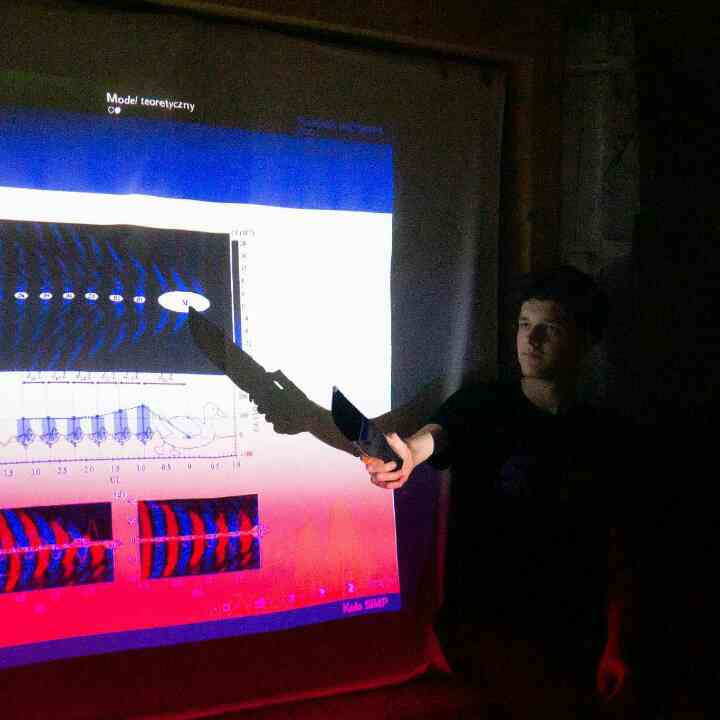
\includegraphics[width=0.5\textwidth]{images/2025-11-13-14-15-37.png}
 \caption{Choć ciężko w to uwierzyć, tez kiedyś byłem młody}
 \end{figure}
\end{frame}

\begin{frame}{Konkluzja}
2021

    PHYSICS PRIZE [THE NETHERLANDS, ITALY, TAIWAN, USA]:
Alessandro Corbetta, Jasper Meeusen, Chung-min Lee, Roberto Benzi, and Federico Toschi, for conducting experiments to learn why pedestrians do not constantly collide with other pedestrians.

REFERENCE: \fullcite{Corbetta_Meeusen_Lee_Benzi_Toschi_2018}

WHO TOOK PART IN THE CEREMONY: Alessandro Corbetta, Jasper Meeusen, Chung-min Lee, Roberto Benzi,, Federico Toschi
\end{frame}

\section{Kiedy ludzie istnieją bez kontekstu}

\begin{frame}{}
\begin{figure}
 \centering
 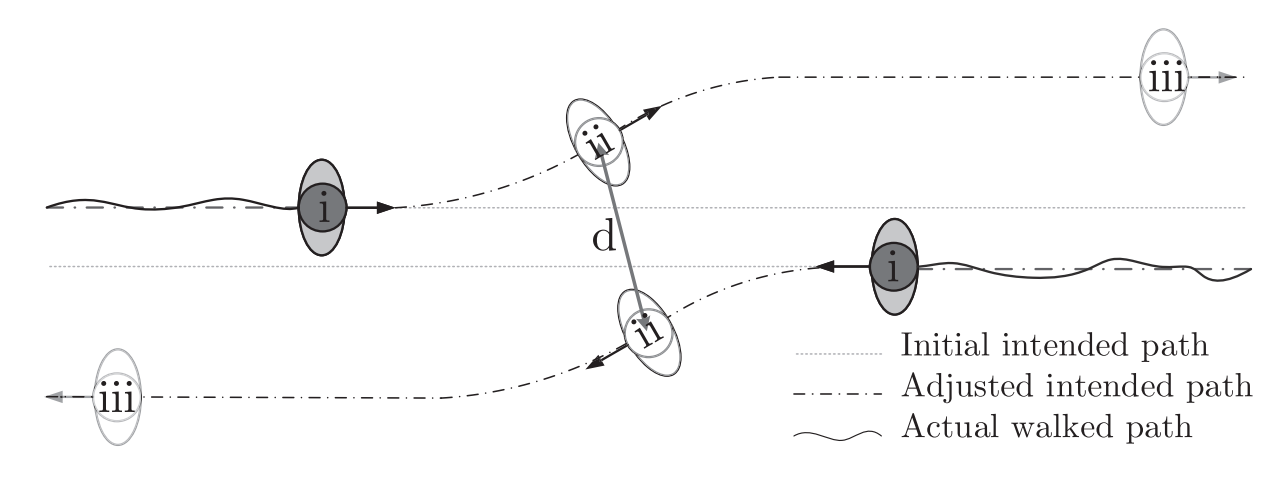
\includegraphics[width=0.9\textwidth]{images/2025-11-13-13-52-03.png}
 \caption{}
 \end{figure}

\end{frame}

\begin{frame}
    \begin{figure}
 \centering
 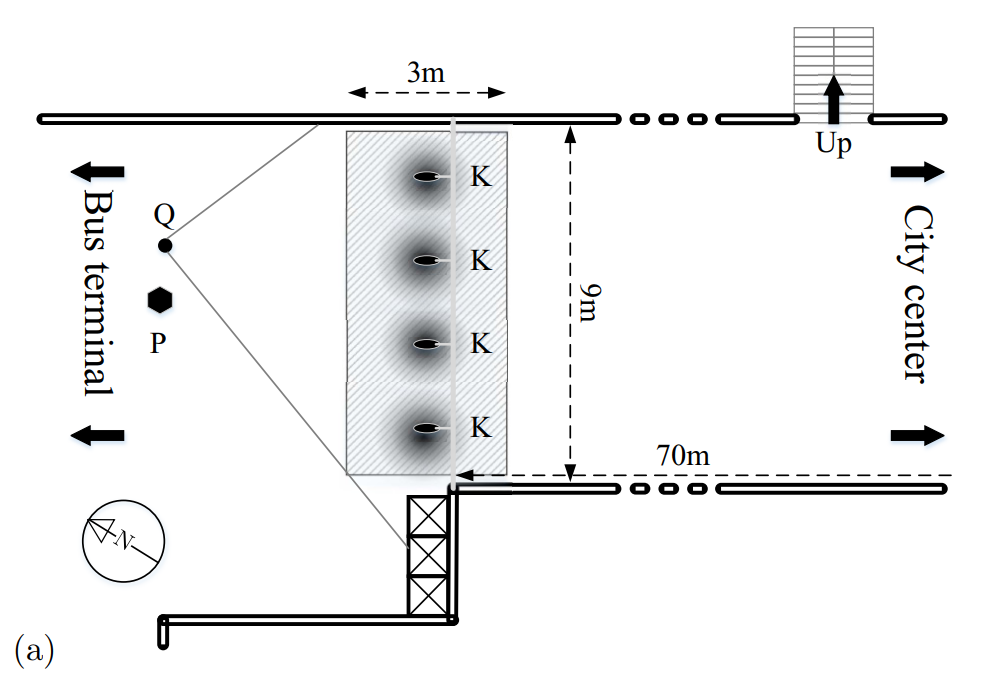
\includegraphics[width=0.49\textwidth]{images/2025-11-13-14-22-09.png}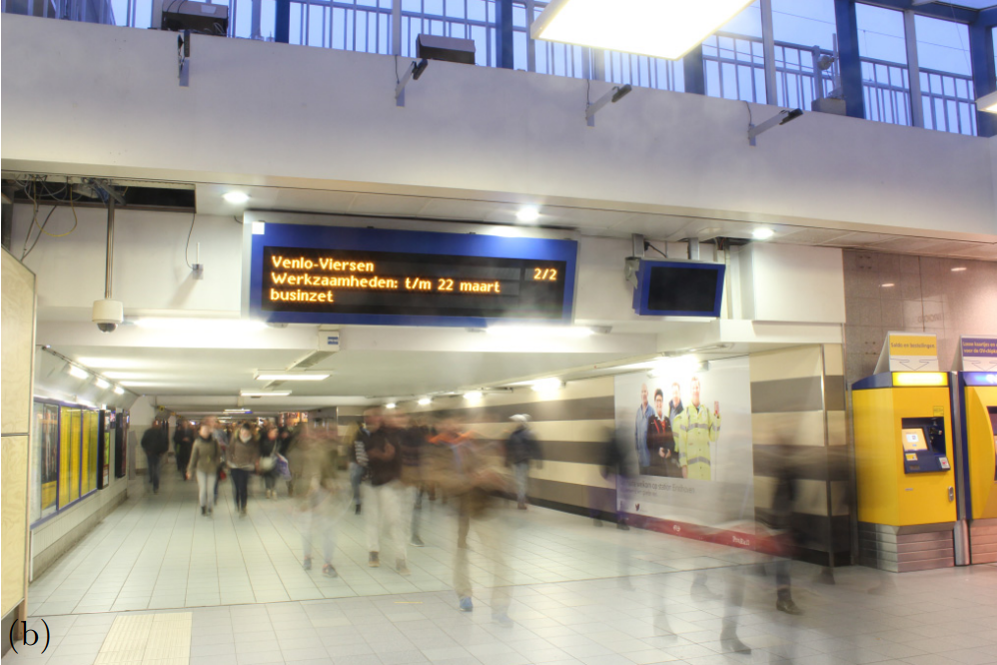
\includegraphics[width=0.49\textwidth]{images/2025-11-13-14-23-37.png}
 \caption{Układ doświadczalny: dworzec kolejowy w Eindhoven. Zacieniowane zostało pole pomiarowe z czterema Kinectami}
 \end{figure}
\end{frame}

\begin{frame}{Wyniki eksperymentu: niezakłócone indywidua}
  \begin{figure}
 \centering
 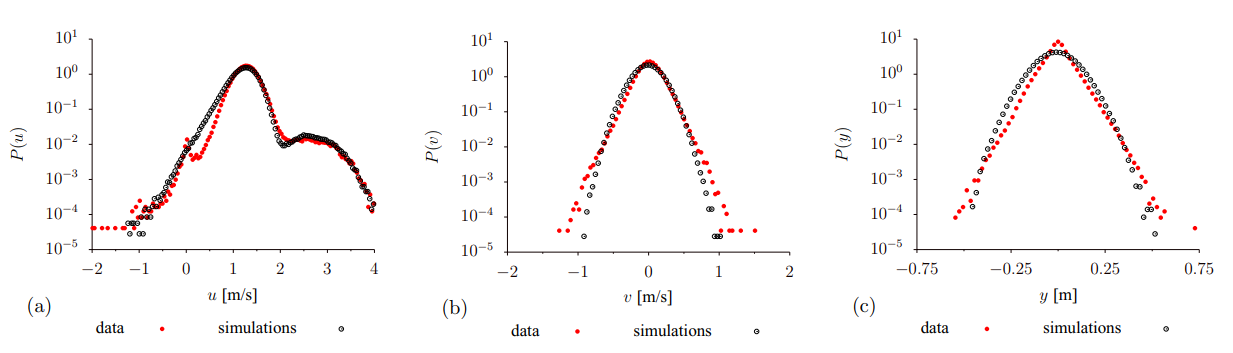
\includegraphics[width=0.95\textwidth]{images/2025-11-13-17-38-14.png}
 \caption{Rozkład prawdopodobieństwa (log-lin) dla: a) prędkości podłużnej $u$, b) prędkości poprzecznej $v$, c) względnego położenia poprzecznego $y$ dla pojedynczych (niezakłóconych) pieszych.}
 \end{figure}
\end{frame}

\section{Kiedy ludzie wchodzą w interakcje}

\begin{frame}{}
  \begin{figure}
 \centering
 \begin{columns}
 \column{0.5\textwidth}
 \centering
 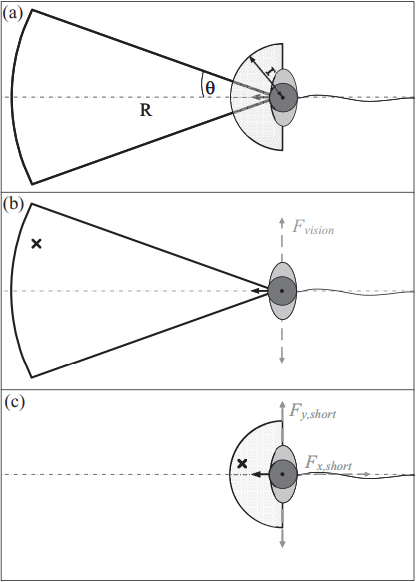
\includegraphics[width=0.85\textwidth]{images/2025-11-13-19-12-20.png}
 \column{0.5\textwidth}
 \caption{Schemat rodzajów siły oddziaływania:}

 b) dalekozasięgowych, opartych na wzroku
 $$\protect F_{vision}=\sgn(e_y)A\exp\left(-\frac{d^2}{R^2}\right)\chi_1(\protect\tilde\theta)$$
 c) krótkozasięgowych
 \[F_{short}=B \exp\left(-\frac{d^2}{r^2}\right)\chi_2(\tilde\theta)\]
%  dupa
%  }
 \end{columns}
\end{figure}
 \end{frame}

\begin{frame}{}
  \begin{figure}
 \centering
 \begin{columns}
 \column{0.5\textwidth}
 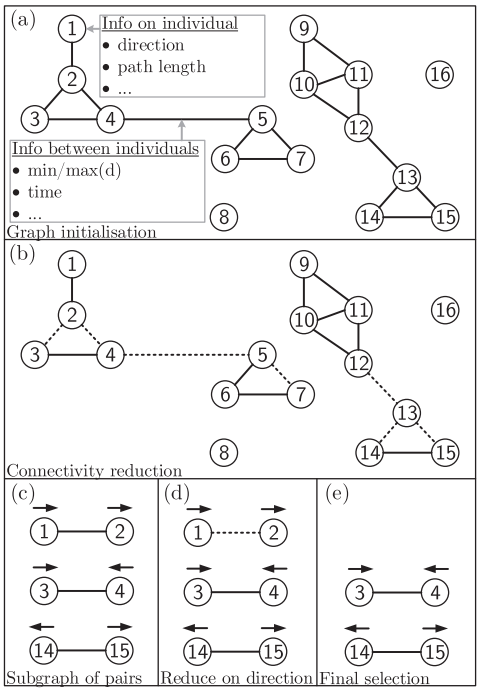
\includegraphics[width=0.85\textwidth]{images/2025-11-14-12-14-09.png}
 \column{0.5\textwidth}
 \caption[foo]{Proces przygotowania grafu interakcji.
 \begin{enumerate}[a)]
  \item inicjalizacja
  \item \emph{sparsing} -- usuwanie krawędzi nie odpowiadających za oddziaływania
  \item odparowywanie -- zostawiamy tylko pary
  \item redukcja ze względu na kierunek
 \end{enumerate}
 }
 \end{columns}
 \end{figure}
\end{frame}

\begin{frame}{}
  \begin{figure}
 \centering
 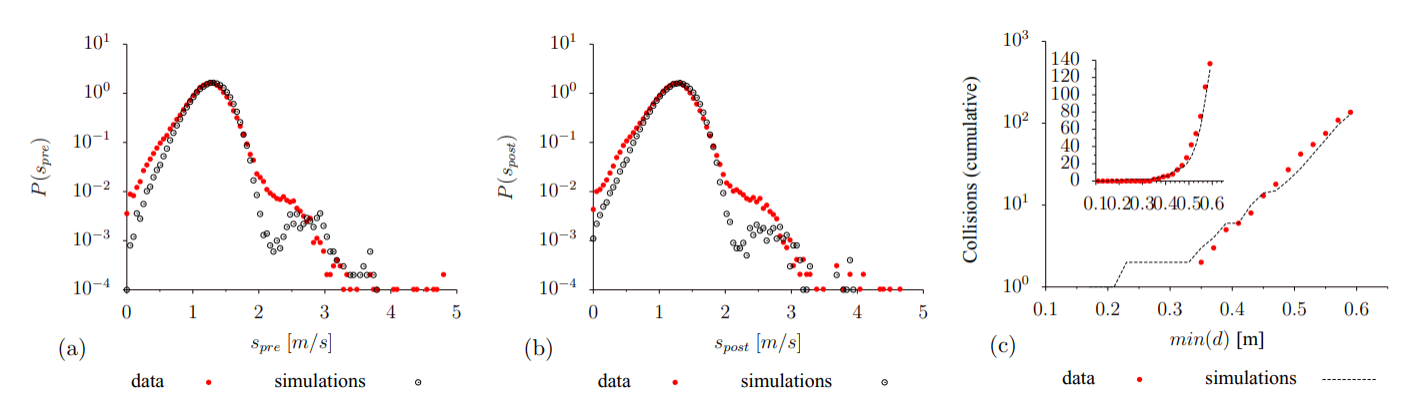
\includegraphics[width=0.95\textwidth]{images/2025-11-14-01-38-01.png}
 \caption{}
 \end{figure}
\end{frame}

\section{Finito}

\begin{frame}{Wnioski}
  \begin{itemize}[<+->]
    \item metoda działa
    \begin{itemize}
      \item ludzie mają oczy
    \end{itemize}
    \item fizyka działa
  \end{itemize}
\end{frame}

\begin{frame}{Twierdzenie (Romuald Jamnik)}
    \begin{figure}
 \centering
 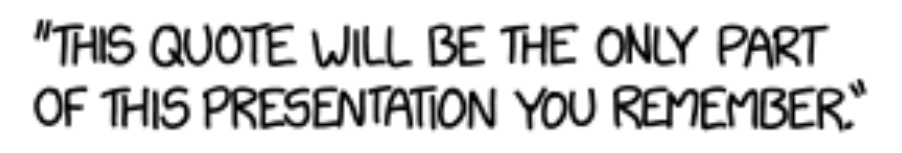
\includegraphics[width=0.6\textwidth]{images/2025-11-13-00-34-41.png}
 \end{figure}
 \begin{figure}
 \centering
 \hspace{0.25\textwidth}
\includegraphics[width=0.3\textwidth]{images/2025-11-13-00-35-06.png}
 \end{figure}
\end{frame}



\end{document}